% Autor: Francisco Javier Barranco Tena
% Experimentos realizados en el desarrollo del TFG
% Alt + z o Option + z para activar el word wrap en Visual Studio Code

Este capítulo se centra en los experimentos realizados durante el desarrollo de este TFG. Para cada experimento se detallarán los pasos seguidos, los resultados obtenidos y las conclusiones extraídas. El TFG se ha realizado de forma iterativa, aplicando las conclusiones de cada experimento a los siguientes hasta llegar a un modelo base que pueda generalizar sobre imágenes de pavimentos.


\section{Experimento 1: Entrenamiento con datos de Estados Unidos y validación cruzada}\label{SEC:EXP1}

El primer experimento relevante que se ha realizado en este TFG ha sido el entrenamiento de un modelo YOLOv8 con los datos de Estados Unidos de la CRDDC2022 y la validación cruzada de 4 \textit{folds}. En total se han realizado 4 iteraciones, una por cada \textit{fold}, y se han obtenido métricas de evaluación para cada iteración. El entrenamiento se ha llevado a cabo en Google Colab con una GPU Tesla T4 y ha durado aproximadamente 1 hora y 40 minutos por iteración. A continuación se detallan los pasos seguidos, los resultados obtenidos y las conclusiones extraídas.

Se ha optado por entrenar solo con los datos de Estados Unidos porque como se puede ver en la tabla \ref{tab:dataset_info}, es una región con una cantidad moderada de imágenes pero con una gran cantidad de anotaciones. Por lo tanto, se considera que es una región adecuada para entrenar un primer modelo y probar la metodología de validación cruzada propuesta. Además, se ha utilizado un modelo YOLOv8 de tamaño \textit{small} y pre entrenado con el conjunto de datos, COCO ('yolov8s.pt'). Se ha utilizado un tamaño de batch de 50 durante 60 épocas para cada iteración. Estos hiperparámetros se han elegido para ajustarse a las limitaciones de memoria de la GPU Tesla T4 de Google Colab y para que el entrenamiento no dure demasiado tiempo.

El objetivo de este experimento es comprobar si la metodología de validación cruzada propuesta es adecuada para evaluar los modelos, ver cuanto podemos aproximarnos a los resultados de la CRDDC2022. Para este primer experimento se ha usado un tamaño de modelo \textit{small} y un subconjunto pequeño de datos para poder iterar rápidamente y extraer conclusiones que se puedan aplicar a futuros modelos más costosos en tiempo y recursos.

Una vez entrenado el modelo, hemos descargado los pesos y se ha realizado la validación de cada modelo con su correspondiente conjunto de validación. Para ello, se ha utilizado el notebook 'validate\_YOLO\_model.ipynb' que se puede encontrar en el repositorio del TFG \cite{TFG_Repository}. Los resultados completos de esta validación para cada iteración se pueden ver en el anexo \ref{CAP:RES_EXP}. La tabla \ref{tab:exp1_results} muestra un resumen de los resultados obtenidos en cada iteración.

\begin{table}[H]
    \centering
    \begin{tabular}{|c|c|c|c|c|}
        \hline
        \textbf{Iteración} & \textbf{Precisión} & \textbf{Recall} & \textbf{F1-score} & \textbf{mAP50} \\ \hline
        0       & 0.630 & 0.685 & 0.656 & 0.706 \\ \hline
        1       & 0.641 & 0.716 & 0.676 & 0.705 \\ \hline
        2       & 0.680 & 0.677 & 0.678 & 0.717 \\ \hline
        3       & 0.662 & 0.675 & 0.668 & 0.711 \\ \hline
        Media   & 0.653 & 0.688 & 0.670 & 0.710 \\ \hline
    \end{tabular}
    \caption{Resultados obtenidos en cada iteración del experimento 1.}
    \label{tab:exp1_results}
\end{table}

Adicionalmente, se han realizado predicciones para las imágenes de test de Estados Unidos y se han subido a la plataforma de la CRDDC2022 para obtener un f1-score sobre los datos de test para los que no tenemos ground truth. Las predicciones se han realizado con el notebook 'predict\_YOLO\_model.ipynb' y usando el modelo que usaba el fold 0 como conjunto de validación. El f1-score obtenido ha sido, \textbf{0.515}, lo que indica que el modelo generaliza bien a datos que no ha visto durante el entrenamiento. En la tabla \ref{tab:top10_f1_scores} se pueden ver los 10 primeros equipos en la plataforma de la CRDDC2022 para los datos de test de Estados Unidos en el momento del cierre de la competición. Los f1-scores están entre 0.726 y 0.844, por lo que podemos concluir que el modelo tiene mucho margen de mejora pese a obtener resultados aceptables.

% Resultados para Estados Unidos en el momento del cierre de la competición
\begin{table}[H]
    \centering
    \resizebox{0,6\textwidth}{!}{
        \begin{tabular}{|c|l|r|}
        \hline
        \textbf{Rank} & \textbf{Team ID} & \textbf{F1-Score} \\ \hline
        1  & T22\_043\_maybe\_he                  & 0.8443163877126995 \\ \hline
        2  & T22\_030\_SH\_S\_U                   & 0.8170061339986036 \\ \hline
        3  & T22\_032\_Dongjun\_Jeong             & 0.8008152493212433 \\ \hline
        4  & T22\_035\_Shouxing\_Wang             & 0.7793253573066574 \\ \hline
        5  & T22\_018\_Ammar\_Mohammed\_Almasrwhi & 0.7788579921283062 \\ \hline
        6  & T22\_014\_Poonam\_Kumari\_Saha       & 0.7751306857212417 \\ \hline
        7  & T22\_022\_Seon\_Ho\_Kim              & 0.7744267351552836 \\ \hline
        8  & T22\_034\_han\_shi\_hao              & 0.743062760430727  \\ \hline
        9  & T22\_024\_yi\_lia\_lia               & 0.7329269630149433 \\ \hline
        10 & T22\_029\_hualin\_he                 & 0.7268546786507959 \\ \hline
        \end{tabular}
    }
    \caption{F1-scores para los 10 primeros equipos en la plataforma de la CRDDC2022 para los datos de test de Estados Unidos en el momento del cierre de la competición.}
    \label{tab:top10_f1_scores}
\end{table}

Se debe considerar que este experimento se ha realizado con un modelo YOLOv8 de tamaño \textit{small} y los modelos solo se han entrenado con un 75\% de los datos anotados de Estados Unidos. Una manera de mejorar el modelo sería entrenar con todos los datos anotados de Estados Unidos y con un modelo YOLOv8 de mayor tamaño.

Otra consideración importante para contextualizar estos resultados es que el ground truth de la CRDDC2022 no es perfecto. Es decir, existen daños en el pavimento que no han sido anotados, por lo que algunas de las predicciones del modelo se evalúan como falsos positivos cuando en realidad sí están indicando un daño real. Además, la CRDDC2022 evalúa cinco predicciones por imagen y el resto las ignoran. En este caso se ha optado por evaluar las cinco predicciones con mayor confianza, pero esto no quiere decir que solo existan esos cinco daños en la imagen. Estas limitaciones de la CRDDC2022 indican que el f1-score obtenido en el experimento 1 es una estimación conservadora de la capacidad de generalización del modelo.

En las figuras \ref{fig:ground_truth_example_1} y \ref{fig:ground_truth_example_4} se pueden ver ejemplos de imágenes donde el ground truth no está completo y el modelo genera anotaciones que pese a ser correctas, no se evalúan como tal en la plataforma de la CRDDC2022. Estos ejemplos ilustran las limitaciones del ground truth y la evaluación de la CRDDC2022. El ejemplo de la figura \ref{fig:ground_truth_example_4} muestra también un caso donde el modelo genera varias anotaciones más pequeñas además de la anotación grande que vemos en el ground truth. Estas anotaciones pese a ser correctas son pequeñas y por lo tanto tendrán un pobre IoU con el ground truth, lo que hace que no se evalúen como correctas en la plataforma de la CRDDC2022, lo que penaliza el f1-score del modelo.

% Añadimos img/ground_truth_example_1.png y img/ground_truth_example_4.png
\begin{figure}[H]
    \centering
    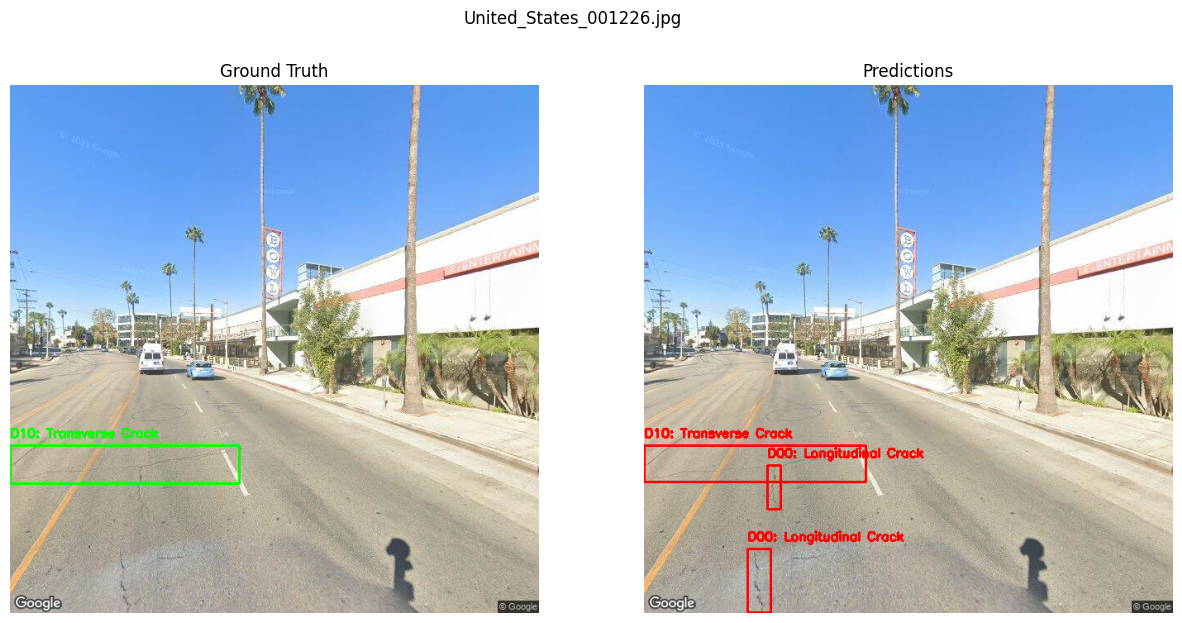
\includegraphics[width=0.8\textwidth]{img/ground_truth_example_1.png}
    \caption{Ejemplo en el que al ground truth le faltan anotaciones. A la derecha, se puede ver que el modelo ha detectado dos grietas longitudinales que no aparecen en el ground truth.}
    \label{fig:ground_truth_example_1}
\end{figure}

\begin{figure}[H]
    \centering
    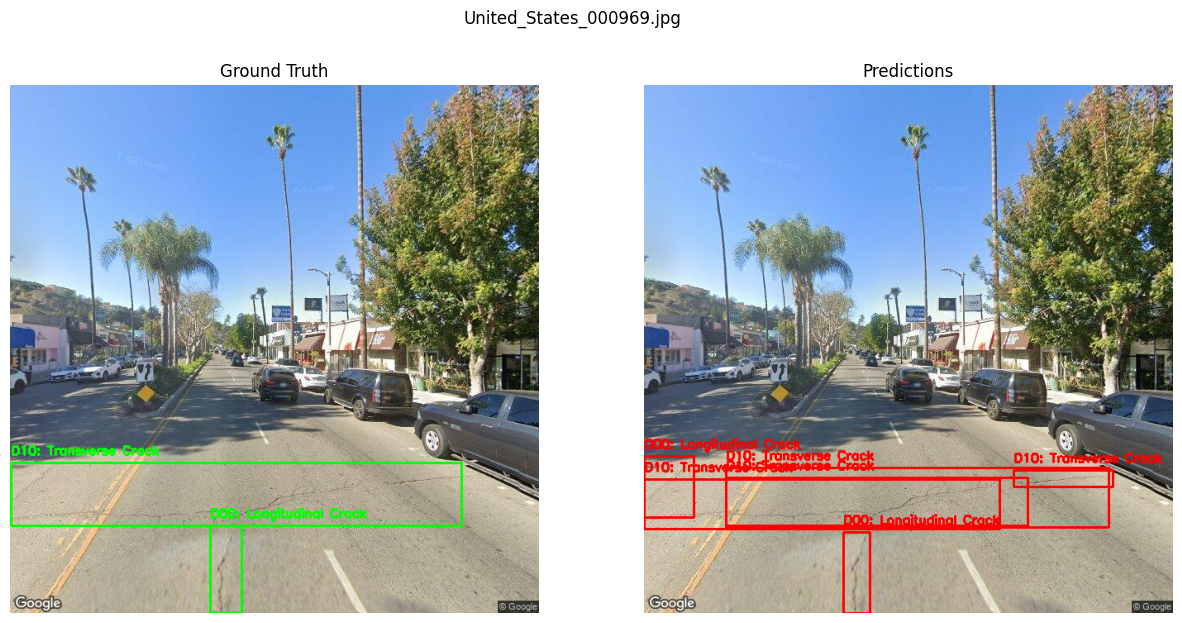
\includegraphics[width=0.8\textwidth]{img/ground_truth_example_4.png}
    \caption{Ejemplo en el que el modelo genera varias anotaciones más pequeñas en lugar de una sola grande, como en el ground truth.}
    \label{fig:ground_truth_example_4}
\end{figure}

En la figura \ref{fig:exp1-cv1-confusion_matrix_normalized} se puede ver la matriz de confusión de la segunda iteración del experimento 1, que es similar a las de las otras iteraciones. En esta matriz de confusión se observa que el modelo detecta la mayoría de las grietas longitudinales, transversales y de piel de cocodrilo del ground truth, pero tiene más problemas con los baches. Esto probablemente se deba a que el conjunto de datos de Estados Unidos tiene pocos ejemplos de baches. Es probable que, al entrenar con todos los datos, el modelo generalice mejor a los baches y aumente la precisión para este tipo de daño. Adicionalmente, en la figura \ref{fig:exp1-cv1-confusion_matrix_normalized} se pueden ver las predicciones de grietas que no aparecen en el ground truth y que penalizan el f1-score del modelo. Como ya se ha mencionado, en muchos casos estas predicciones son correctas pero no aparecen en el ground truth o se han generado varias anotaciones pequeñas en lugar de una grande.

% Añadimos la imagen exp1-cv1-confusion_matrix_normalized.png
\begin{figure}[H]
    \centering
    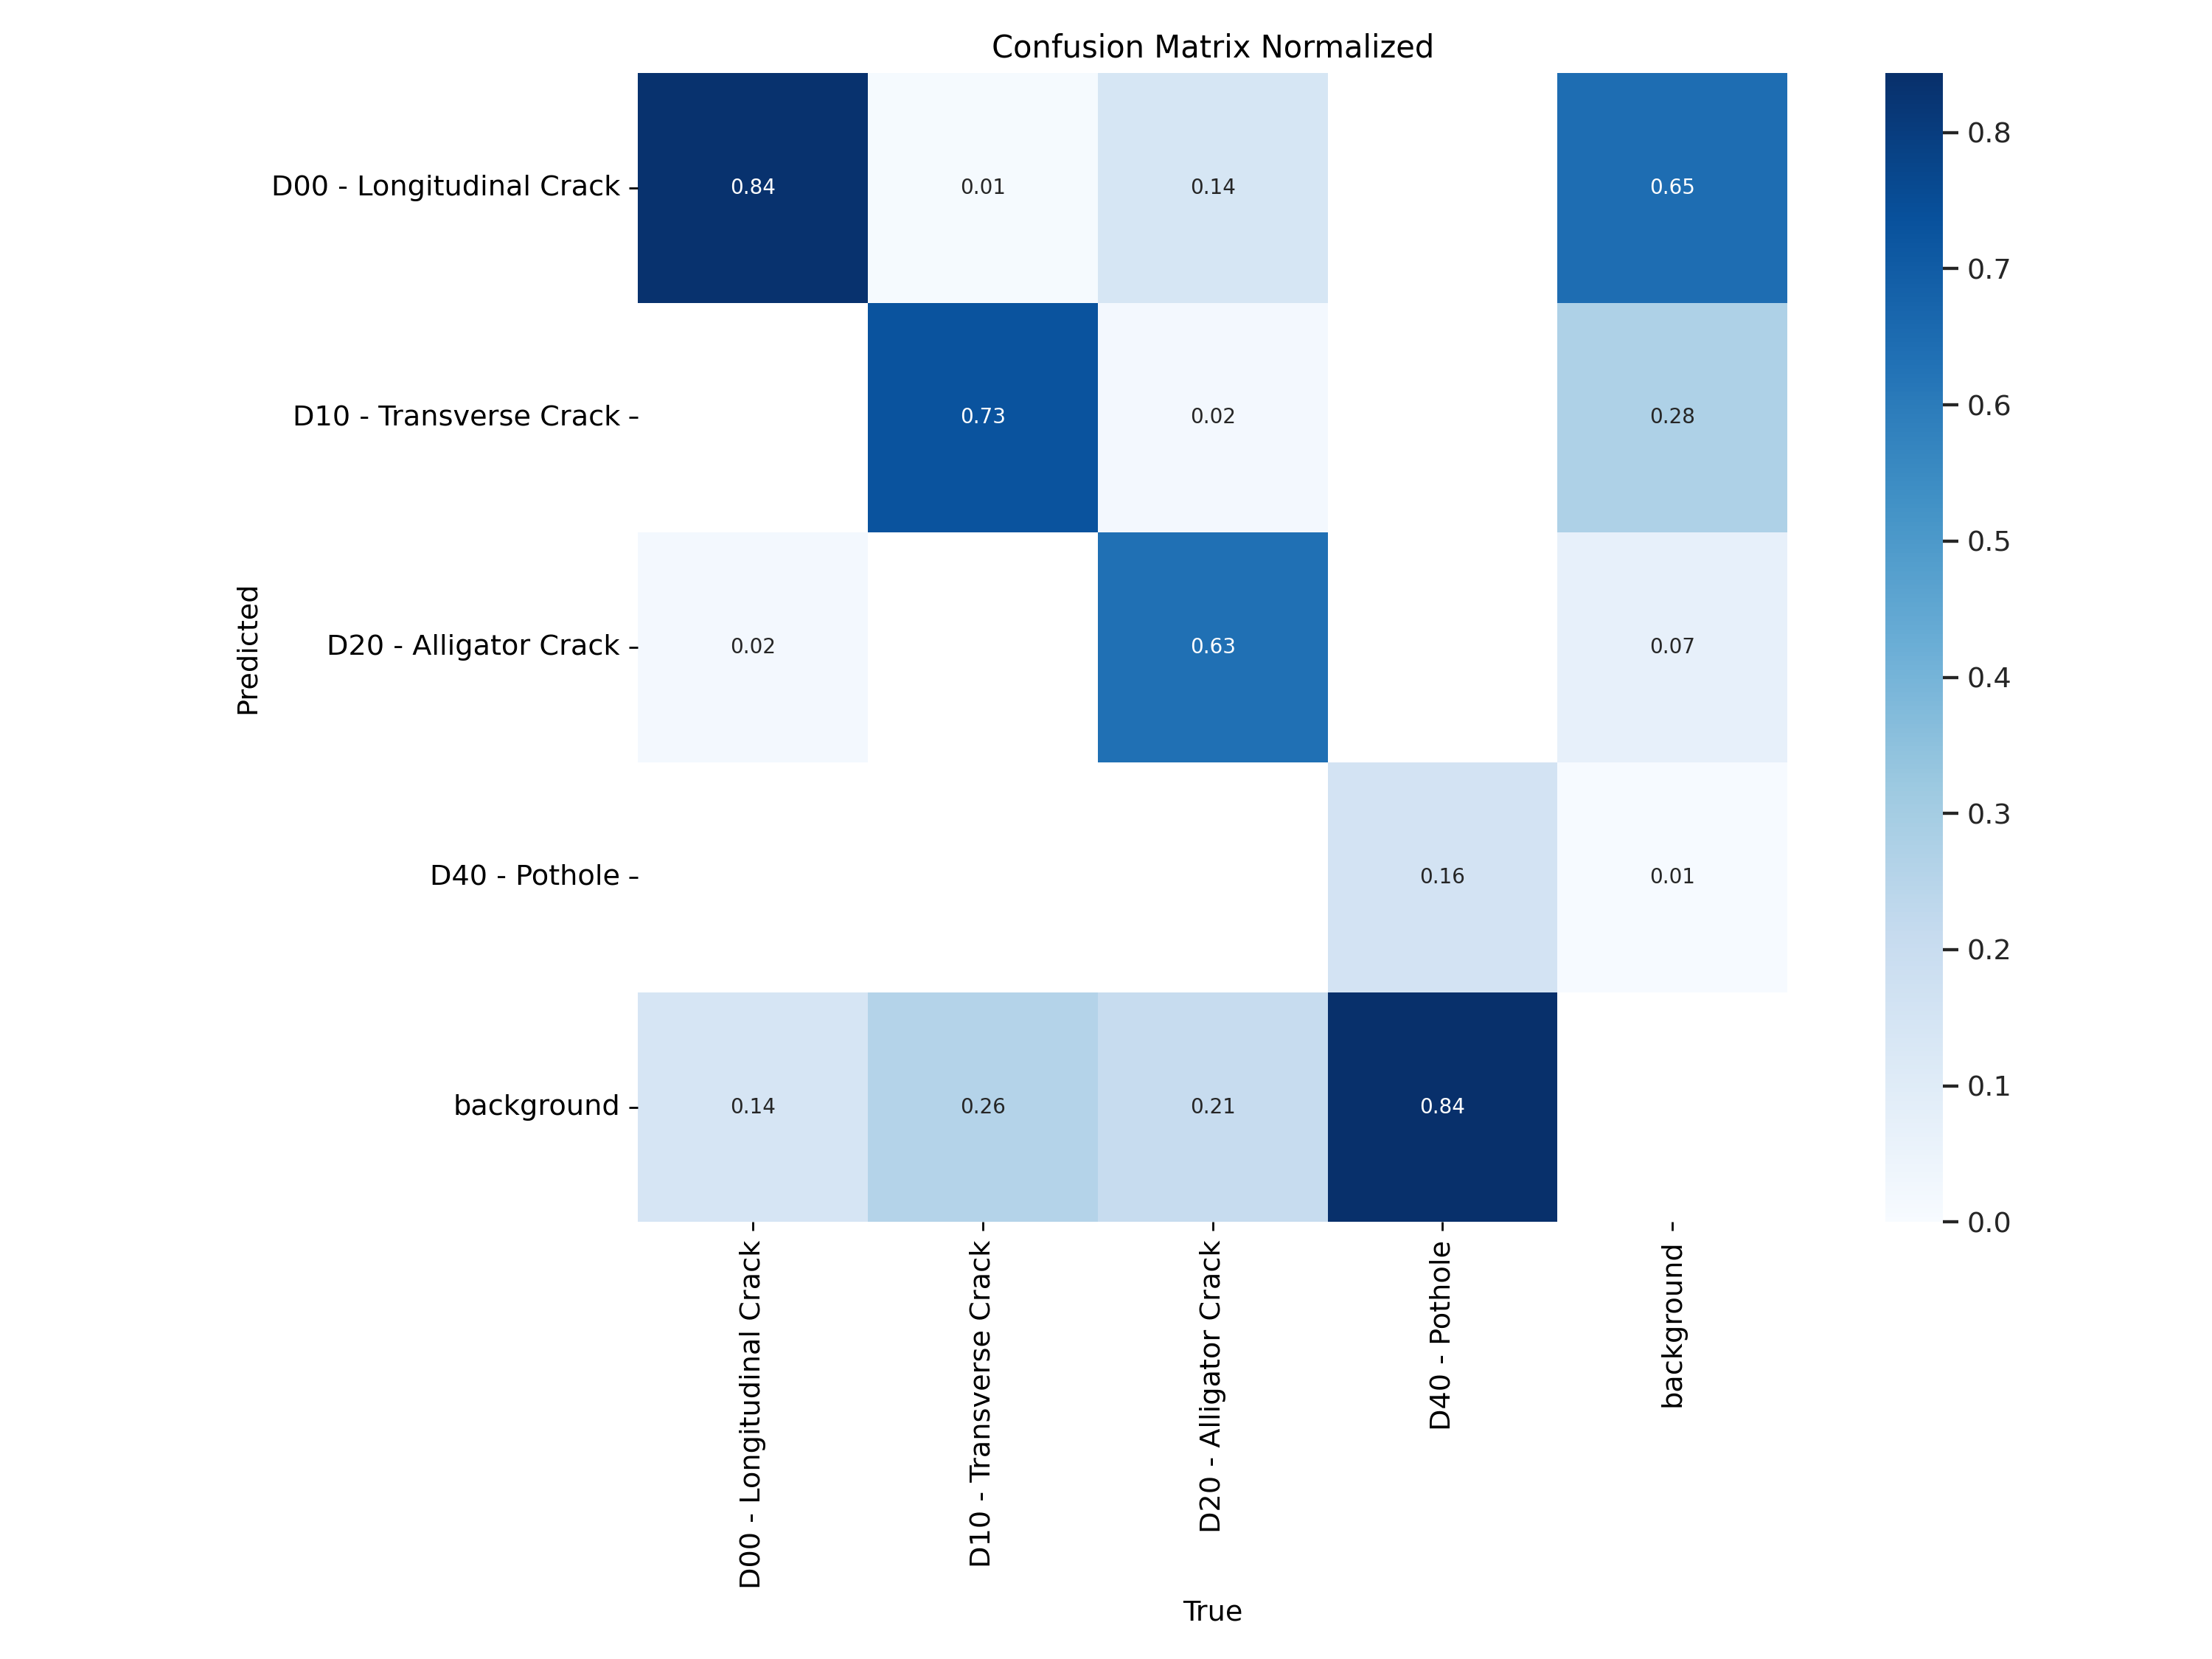
\includegraphics[width=0.9\textwidth]{img/exp1-cv1-confusion_matrix_normalized.png}
    \caption{Matriz de confusión normalizada de la segunda iteración del experimento 1.}
    \label{fig:exp1-cv1-confusion_matrix_normalized}
\end{figure}

\section{Experimento 2: YOLO de mayor tamaño y entrenamiento con todos los datos de Estados Unidos}\label{SEC:EXP2}

Una de las principales conclusiones extraídas del experimento 1 es que probablemente se puede mejorar el rendimiento del modelo si se entrena con todos los datos anotados de Estados Unidos y se utiliza un modelo YOLOv8 de mayor tamaño. Por lo tanto, en este experimento se ha entrenado un modelo YOLOv8 de tamaño \textit{very large} con todos los datos anotados de Estados Unidos. El objetivo de este experimento es comprobar si se puede mejorar el rendimiento del modelo y si se puede obtener un f1-score más alto en la plataforma de la CRDDC2022. Como vamos a usar todos los datos anotados para entrenar, no nos podemos fiar de ninguna validación, ya que inevitablemente se usaran imágenes vistas en entrenamiento para validar. Por lo tanto, no se ha realizado validación cruzada en este experimento.

Se ha utilizado un modelo YOLOv8 de tamaño \textit{very large} y pre entrenado con el conjunto de datos COCO ('yolov8x.pt'). Además, se ha utilizado un tamaño de batch de 15 durante 60 épocas. Estos hiperparámetros se han elegido para ajustarse a las limitaciones de memoria de la GPU Tesla T4 de Google Colab y para que el entrenamiento no dure demasiado tiempo. El entrenamiento ha durado 7 horas. En el anexo \ref{CAP:RES_EXP} se pueden ver el resumen de este entrenamiento generado por Ultralytics.

Una vez entrenado el modelo, se han realizado predicciones para las imágenes de test de Estados Unidos y se han subido a la plataforma de la CRDDC2022 para obtener un f1-score sobre los datos de test para los que no tenemos ground truth. El f1-score obtenido ha sido, \textbf{0.607}, lo cual supone una mejora de casi 18\% respecto al experimento 1.

Adicionalmente a este experimento, se ha realizado un entrenamiento de un YOLOv8 \textit{very large} con el fold 0 como conjunto de validación y el resto como entrenamiento. Se han utilizado 150 épocas y un tamaño de batch de 15. El objetivo de este entrenamiento ha sido ver cuantas épocas son necesarias para que el modelo \textit{very large} converja y si se puede mejorar el f1-score obtenido en el experimento 2. En las gráficas de 'val\/box\_loss' y 'val\/dfs\_loss' de la figura \ref{fig:exp2b-results} se pueden ver que para este entrenamiento con un 75\% de los datos anotados de Estados Unidos, el modelo converge en aproximadamente 90 épocas y a partir de ahí comienza a sobreajustar. De esto se puede concluir que el experimento 2 con un 100\% de los datos anotados de Estados Unidos y 60 épocas quizás podría haberse beneficiado de más épocas de entrenamiento.

% Añadir la imagen exp2b-results.png
\begin{figure}[H]
    \centering
    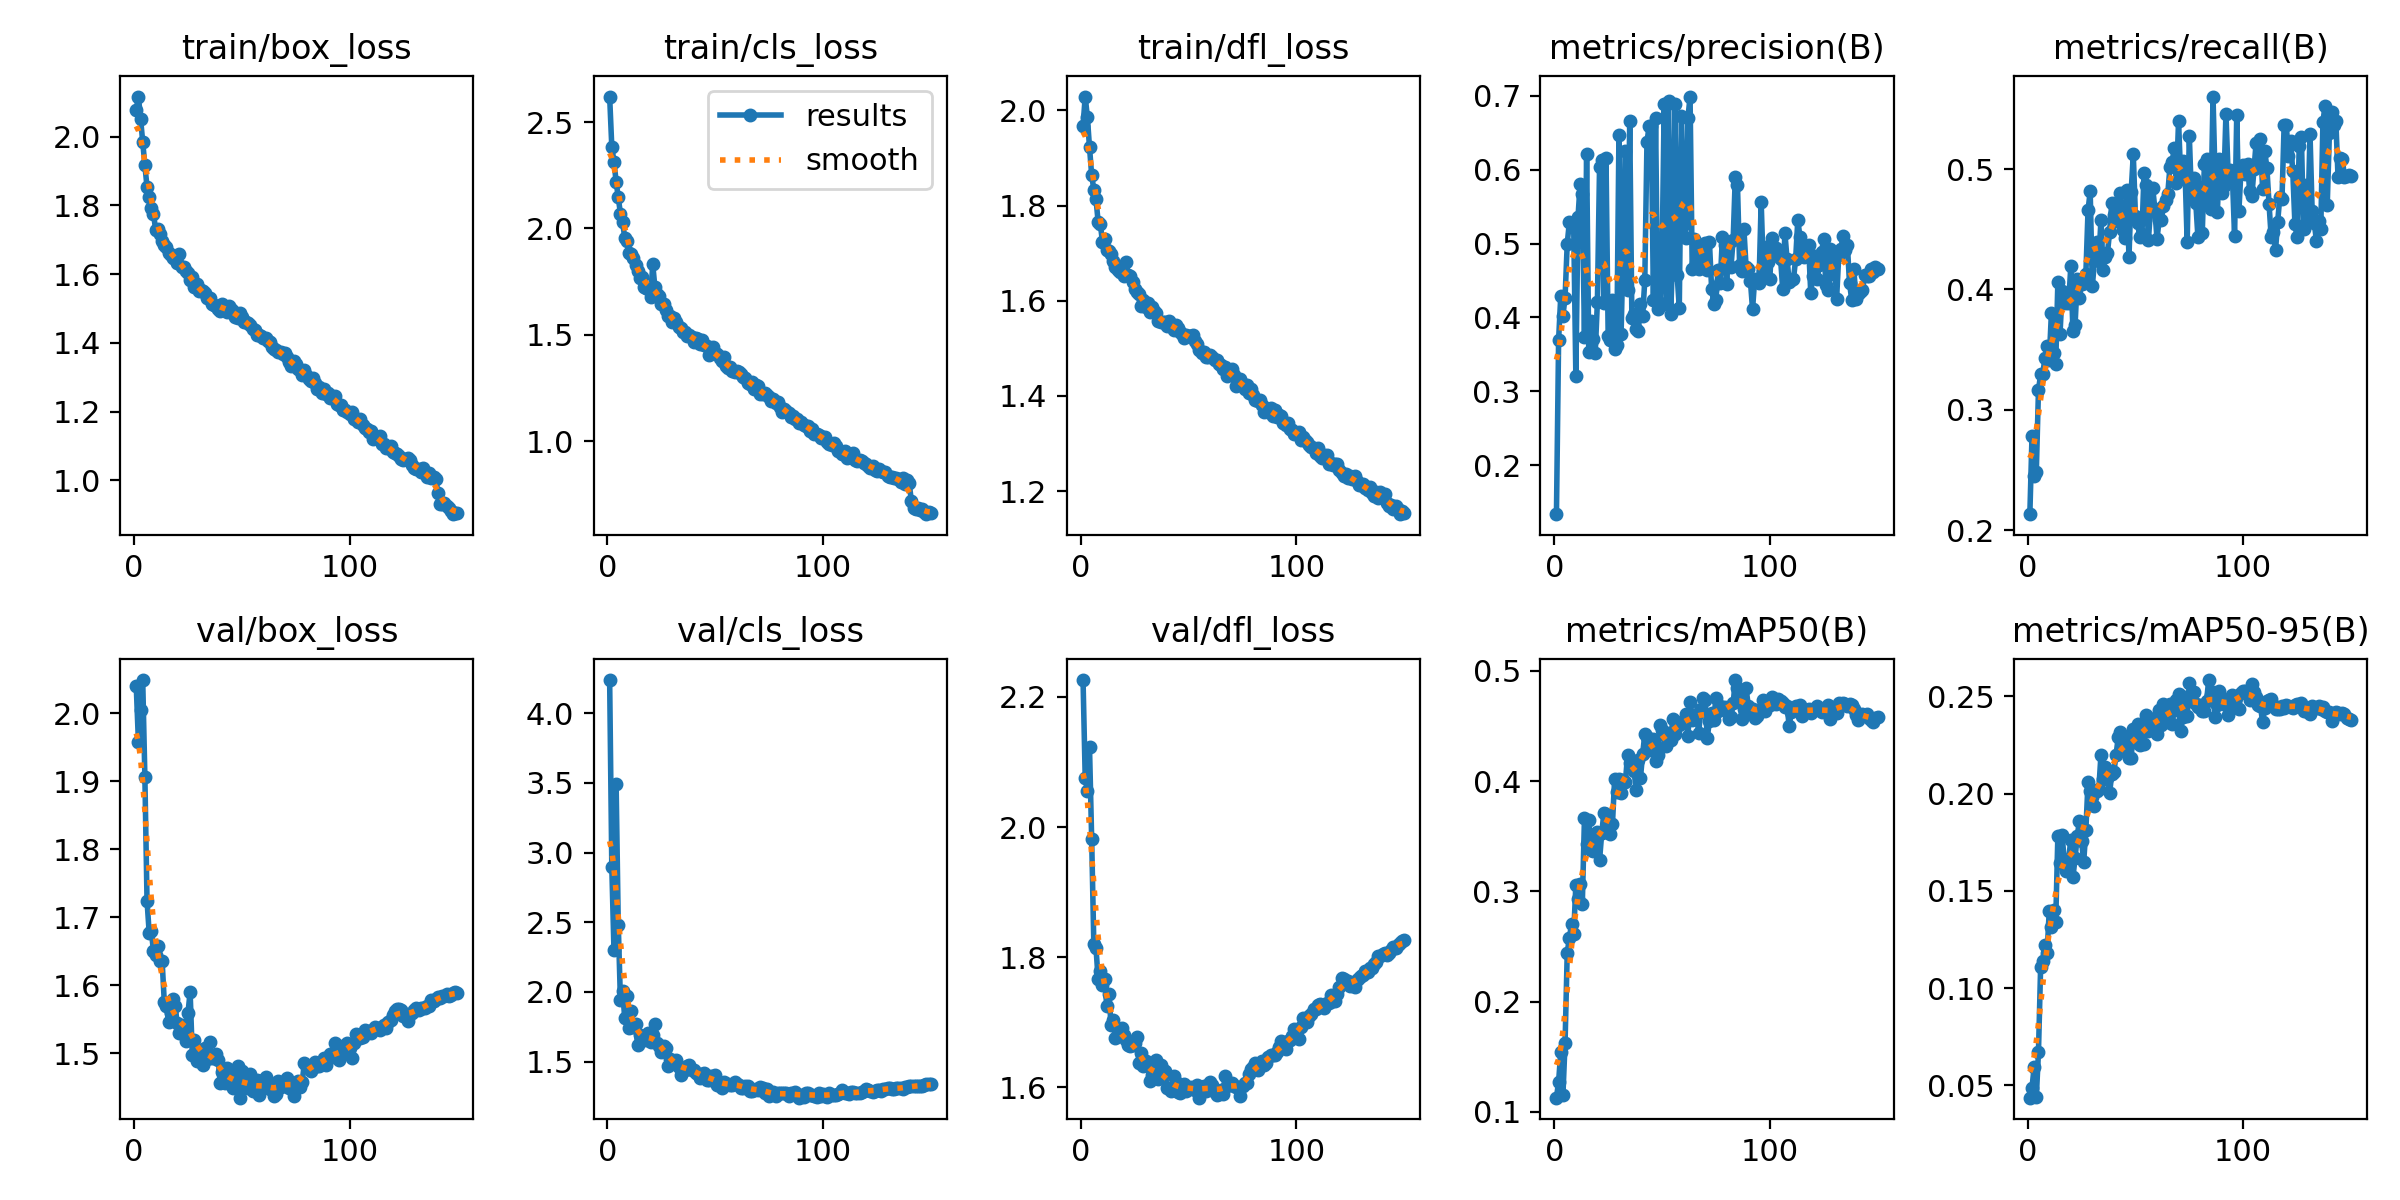
\includegraphics[width=0.9\textwidth]{img/exp2b-results.png}
    \caption{Resultados del entrenamiento del modelo YOLOv8 \textit{very large} con el fold 0 como conjunto de validación.}
    \label{fig:exp2b-results}
\end{figure}

Se ha intentado aplicar esta conclusión para mejorar el f1-score del experimento 2 extendiendo el entrenamiento con el 100\% de los datos de entrenamiento de 60 a 120 épocas. Sin embargo, el f1-score obtenido en la plataforma ha sido de \textbf{0.604}, casi el mismo que en el experimento 2. Esto indica que el modelo o bien ya convergía en 60 épocas o bien pierde f1-score por sobreajuste con 120 épocas. Como se han usado todos los datos de entrenamiento, no se puede saber si el modelo ha sobreajustado mirando los resultados de validación.


\section{Experimento 3: Entrenamiento con todos los conjuntos de datos y validación simple}\label{SEC:EXP3}

En este experimento, se ha entrenado un modelo YOLOv8 de tamaño \textit{very large} con todos los conjuntos de datos de la CRDDC2022. Se ha realizado una validación simple utilizando el 75\% de los datos para entrenamiento y el 25\% para validación, sin utilizar validación cruzada debido a la alta demanda computacional de este experimento.

Debido al tamaño del modelo \textit{very large}, el mayor tamaño de batch soportado por las Tesla T4 de Google Colab era 16. Con 28784 imágenes de entrenamiento y 9601 de validación, el tamaño de batch de 16 resultaba en 1799 iteraciones de entrenamiento y 601 de validación por época. Ejecutando este proceso en Google Colab con una Tesla T4, cada época duraba aproximadamente 43 minutos. Esto significa que un entrenamiento de 60 épocas duraba aproximadamente 43 horas. Por lo tanto, no era razonable realizar una validación cruzada simplemente para garantizar una ligera mejora en la generalización del modelo.

Los pesos de los modelos entrenados en Google Colabs se han descarcago y se ha realizado la inferencia en local sobre los distintos conjuntos de datos que componen la CRDDC2022. Los resultados obtenidos en la plataforma de la CRDDC2022 se pueden ver en la tabla \ref{tab:exp3_results}.

\begin{table}[H]
    \centering
    \resizebox{0,4\textwidth}{!}{
        \begin{tabular}{|l|r|}
        \hline
        \textbf{Conjunto de Datos} & \textbf{F1-Score} \\ \hline
        Todos           & 0.596914344950027     \\ \hline
        India           & 0.37469955667942845   \\ \hline
        Japón           & 0.5946284828735682    \\ \hline
        Noruega         & 0.3097122625784419    \\ \hline
        Estados Unidos  & 0.6412266602062118    \\ \hline
        \end{tabular}
    }
    \caption{F1-scores obtenidos en la plataforma de la CRDDC2022 para los distintos conjuntos de datos.}
    \label{tab:exp3_results}
\end{table}

SIN TERMINAR
SIN TERMINAR
SIN TERMINAR
SIN TERMINAR